\chapter{Problem Statement and Methods}

This chapter serves as a brief, but in-depth summary, concisely detailing the problem. Followed by the Methodology used in this work.

\section{Developing a Sensor Health Monitoring}

Problems with large-scale measuring systems in comparison to smaller experimental setups is the sheer scale and inefficiency of manually checking for errors. Since errors in aviation contexts mostly have fault rates of $10^-6/h$ it allows for some errors during runtime even with large datasets of up to 5000 sensors. However, many sensors in this application are built-in experimentally and can be assumed to be at a fault rate of $1/h$.

This work then shall start with the skystash architecture in mind. Firstly, it needs to be assured that the available data is sensibly imported into the skystash. A second hurdle lies within the metadata treatment. Metadata needs to be parsed from the proprietary .imcexp format. Steps undertaken will then involve uploading the available data to the skystash without modification, forming the first step of data provision.
Metadata enrichment follows as the next step, enriching the DAQ metadata with additional sensor information, SHM information such as boundaries for level 2 as well as level 3 tags for mapping parameters onto categories. Within this step all this data is then taken and transformed into a standardized format (like the SOIL format) that enables a standardized interface to the data processing step.
Data processing builds the next step. The previously standardized, enriched metadata is used to check levels 1, 2 and 3 as presented in chapter 2. For Level 1 (Completenss) the challenge lies in accessing the configuration for expected sensor values. For Level 2 (Plausibility), statistical methods will be used to examine single sensors for plausible behavior such as noise and hard limits. In Level 3 (Correctness), the correlation of parameters has to be made to detect if sensors deviate strongly from other sensors measuring the same value. Also a way has to be found to implement physical relations.
Building a visualization of the reported parameters is the next step. Here, a User Interface will be implemented to give a high information density, allowing users to gain an easy overview but also facilitating trouble shooting by giving a customizable depth of detail.

This work needs to be highly modular to allow parallelisation of tasks and also limit complexity of the codebase. Computing with large flight data sets is time-intensive and modularizing the logic as well as the data allows for easier fixes and better maintainability.

\section{Methodology}

Since SHM is a multifaceted problem that represents a grand undertaking with many moving parts and optimizable parameters, algorithms and systems that may be implemented, it is firstly considered necessary to develop an ecosystem and a process in which SHM algorithms may be tested, evaluated and optimized. To develop said ecosystem, the turbine model for development of Human-Machine Systems is featured (see figure \ref{fig:innovation_turbine}). Its process can be applied to this work without much change. Starting from Ideation stage that represents the beginning phase as well as the first Chapter of this work. Within Ideation phase the project orientation takes place. Answering the question of which goals are considered viable within the given constraints of time and manpower as well as ressources such as knowledge and available tooling.
After Ideation Phase the vertical movement representing creativity and innovational ideas is centered into a level-headed assessment of the problem containing goals and boundary conditions. Using these condensed ideas and values, the Research and Technology Assessment Phase is kicked off, represented by Chapter 2 of this work in which various technologies are examined for usage within the given problem context. Based upon a wide and thorough research feasible ideas and approaches can now be arranged within an infrastructure to solve the given problem. Fitting together various approaches from the literature like puzzle-pieces and condensing the ideas into a more refined concept, concluding literature review and representing a first draft. Using this first draft, the development cycle can now be started which can also be represented by the spiral model for development as presented by \textcite{boehm_spiral_1986}. The challenge of this third stage is now to implement the draft given in the previous stage, this gets accomplished by bouncing from an exploration step in which the theoretical constructs from the previous steps are implemented into a review step in which the systems are rated upon usability. This also represents the procedure of chapter 4 in which the theory from chapter 2 is implemented and developed. After having then developed a prototype of this work we can assess the results for our test cases (sensor failures) in chapter 5.




\begin{figure}[h]
    \centering
    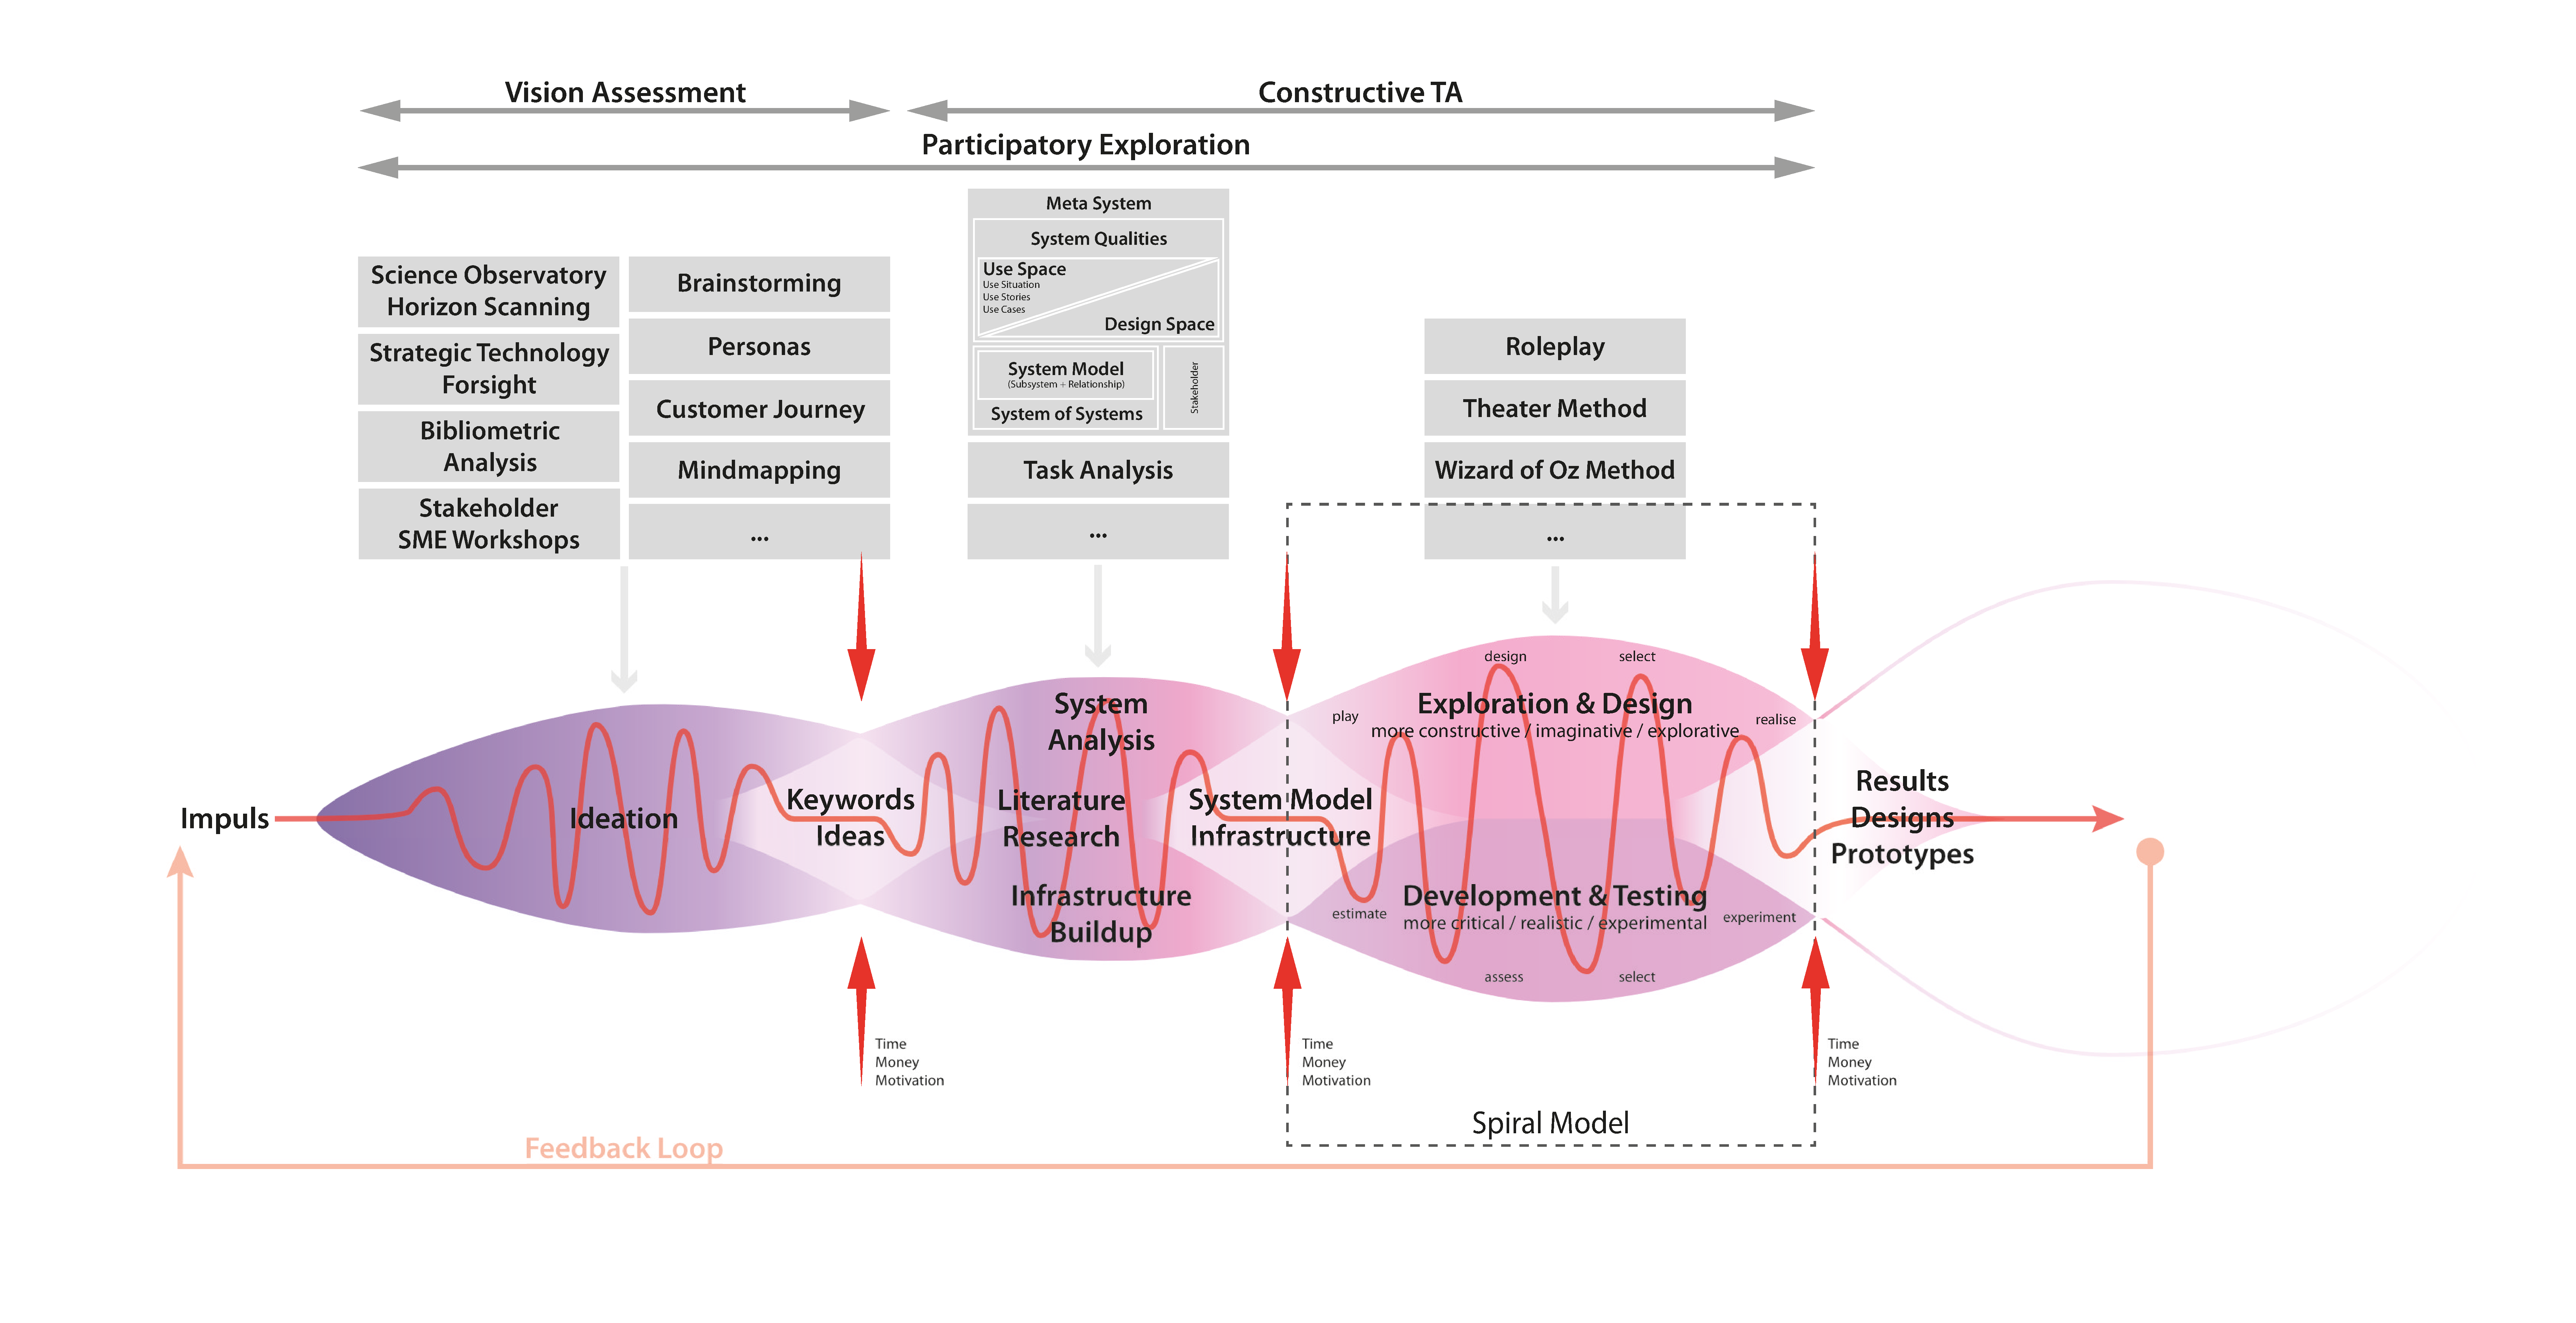
\includegraphics[width=\textwidth]{Innovationsturbine}
    \caption{The innovation and exploration turbine in the context of this work as a two times nested feedback loop. \cite{adlakha-hutcheon_human_2022}}
    \label{fig:innovation_turbine}
\end{figure}

%\begin{figure}[h]
    %\centering
    %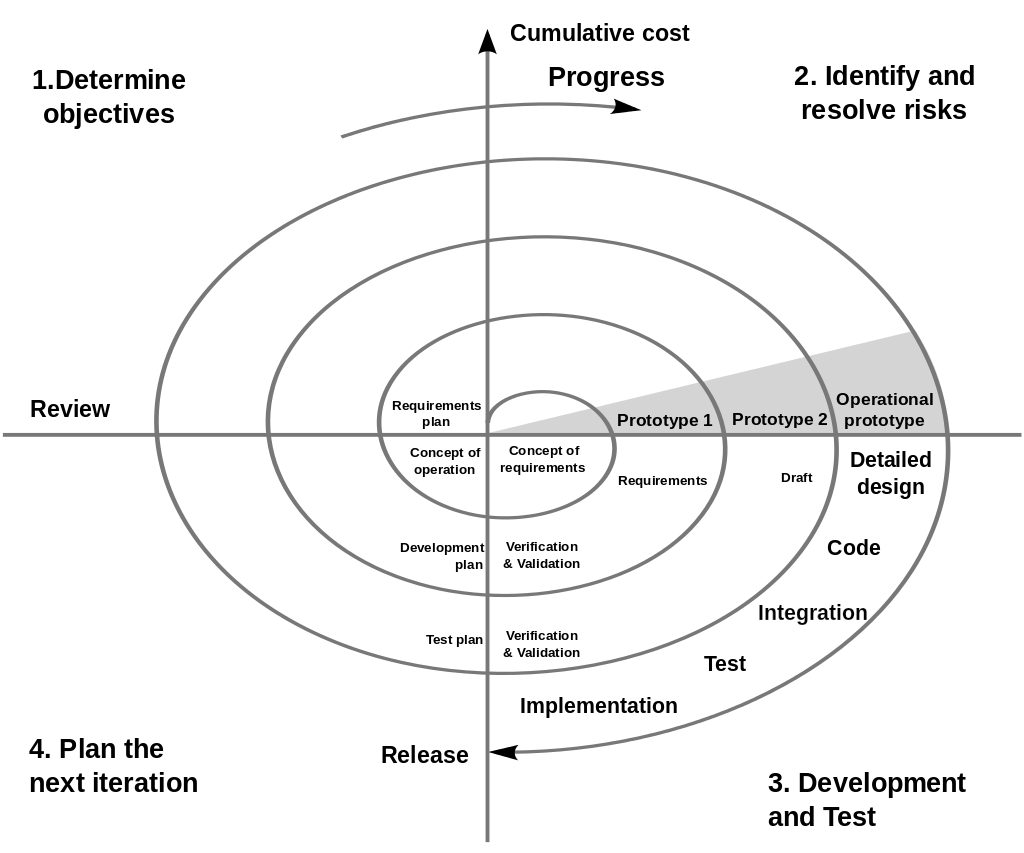
\includegraphics[width=.8\textwidth]{Spiral_model_(Boehm,_1988).svg}
    %\caption{The spiral model featured within the innovation turbine \cite{boehm_spiral_1986}}
    %\label{fig:spiral model}
%\end{figure}


